\documentclass[11pt,a4paper]{article}
\usepackage{float}
\usepackage{tikz}
\usetikzlibrary{arrows.meta, positioning}

\usepackage[T1]{fontenc}
\usepackage[utf8]{inputenc}
\usepackage[margin=2.4cm]{geometry}
\usepackage{amsmath,amssymb}
\usepackage{graphicx}
\usepackage{booktabs}
\usepackage{array}
\usepackage{rotating}      % sidewaystable for the wide results table
\usepackage{caption}
\usepackage{enumitem}
\usepackage{xcolor}
\usepackage{tikz}
\usetikzlibrary{positioning,arrows.meta,shapes.geometric}
\usepackage[hidelinks]{hyperref}

\captionsetup{font=small,labelfont=bf}
\setlist[itemize]{topsep=2pt,itemsep=1pt,parsep=0pt}
\setlist[enumerate]{topsep=2pt,itemsep=1pt,parsep=0pt}

% Tighten the big results table
\newcommand{\tinytable}{\footnotesize\setlength{\tabcolsep}{3.5pt}}

\title{\textbf{Robust Histopathology Image Classification under Staining Variations}}
\author{Deep Learning (DL2026) --- Group 1 · Project 32\\[2pt]
        Repository: \texttt{DL2026-1-32}}
\date{\today}

\begin{document}
\maketitle
\vspace{-1.2em}

% =====================================================================
\section{Abstract}
% =====================================================================
Deep learning models achieve high accuracy in digital histopathology. However, when
these models run on images from another hospital, their performance often drops
sharply. This problem happens because staining chemicals, laboratory protocols, and
slide scanners create large color variations between hospitals. In this project, we
study how to make convolutional and transformer models robust against staining shifts
in colorectal cancer tissue classification. We train models on 24{,}993 patches from
the NCT-CRC-HE-100K-NONORM dataset (Heidelberg cohort) and test them on 7{,}180 unseen
patches from the CRC-VAL-HE-7K dataset (Aachen cohort) across nine tissue classes. We
design a 13-experiment ablation matrix to evaluate three defense axes: color
normalization (Reinhard and Macenko), data augmentation (geometric transformations and
biological HED stain jitter), and model backbones (ResNet-50, ConvNeXt-Tiny, and the
Phikon foundation model). Our experiments reveal three key findings: stain
normalization recovers up to 18 F1 points on external data; stain augmentation becomes
redundant once normalization is applied; and pretrained foundation models show strong
zero-shot stain robustness but suffer when artificial normalization alters their
learned feature distributions. Our best-defended ResNet-50 model achieves an
out-of-domain Macro-F1 score of 0.8689.

% =====================================================================
\section{Introduction and Research Question}
% =====================================================================

\subsection{Clinical Background and Problem Statement}
Colorectal cancer is one of the leading causes of cancer deaths worldwide. In clinical
pathology, doctors examine tissue biopsies under a microscope to confirm diagnosis and
plan patient treatment. To see cellular structures clearly, laboratory technicians
stain thin tissue slices with two chemical dyes: \textbf{Hematoxylin} and
\textbf{Eosin} (H\&E).
\begin{itemize}
  \item \textbf{Hematoxylin} stains cell nuclei deep purple-blue because it binds to
        acidic nucleic acids (DNA and RNA).
  \item \textbf{Eosin} stains the cytoplasm, extracellular matrix, and muscle fibers
        bright pink-red because it binds to basic proteins.
\end{itemize}

Digital pathology scanners convert these glass slides into high-resolution digital
images called Whole Slide Images (WSI). In recent years, Deep Convolutional Neural
Networks (CNNs) and Vision Transformers (ViTs) have shown impressive diagnostic
accuracy on digital slides.

However, a critical barrier stops these AI models from safe clinical deployment:
\textbf{inter-laboratory staining variation}. Even though all hospitals follow
standard H\&E protocols, the visual appearance of slides differs greatly between
medical centers. These color shifts happen due to:
\begin{enumerate}
  \item Different chemical manufacturers, dye purity, and reagent batch ages.
  \item Variations in tissue processing time, fixation quality, and microtome section
        thickness.
  \item Differences in optical lenses, light sources, and sensor color calibration
        across digital slide scanner brands (such as Philips, Leica, or Hamamatsu).
\end{enumerate}

\begin{figure}[h]
\centering
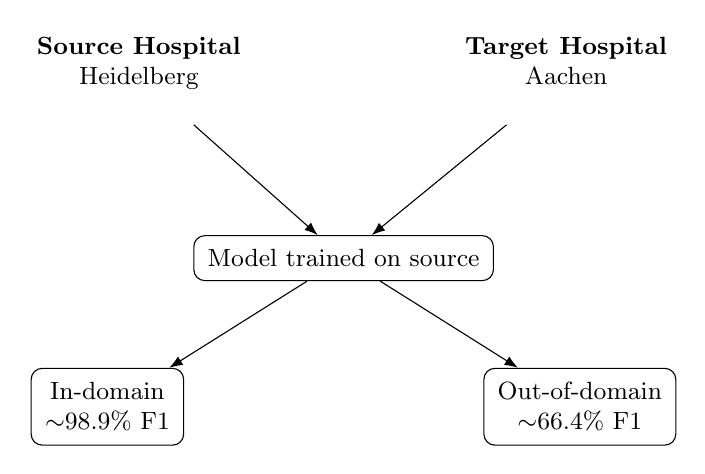
\begin{tikzpicture}[
  node distance=9mm,
  box/.style={draw, rounded corners, align=center, font=\small, inner sep=5pt},
  sm/.style={font=\small, align=center}
]
\node[sm] (src) {\textbf{Source Hospital}\\Heidelberg\\};
\node[sm, right=26mm of src] (tgt) {\textbf{Target Hospital}\\Aachen\\};
\node[box, below=14mm of src, xshift=26mm] (model) {Model trained on source};
\node[box, below=11mm of model, xshift=-30mm] (id) {In-domain\\$\sim$98.9\% F1};
\node[box, below=11mm of model, xshift=30mm]  (ood) {Out-of-domain\\$\sim$66.4\% F1};
\draw[-{Latex}] (src) -- (model);
\draw[-{Latex}] (tgt) -- (model);
\draw[-{Latex}] (model) -- (id);
\draw[-{Latex}] (model) -- (ood);
\end{tikzpicture}
\caption{Domain shift between two clinical centers. A model trained on one hospital
cohort loses a large fraction of its diagnostic performance on an external cohort.}
\label{fig:domainshift}
\end{figure}

\subsection{The Shortcut Learning Challenge}
When a deep learning model trains on images from only one hospital, it easily learns
``shortcuts'' instead of true biological features. For example, if tumor regions at
Hospital A happen to have slightly darker purple tones due to high nuclear density,
the network may simply learn: \textit{``Dark purple means cancer, light pink means
benign tissue''}.

When this model is deployed at Hospital B, where normal muscle tissue is stained
darker purple or cancer tissue is stained lighter pink, the model becomes confused and
fails. In machine learning, this failure is called \textbf{domain shift} or
\textbf{out-of-distribution (OOD) degradation}. In clinical medicine, such errors can
lead to missed tumors or false cancer diagnoses.

\subsection{Research Questions}
To understand what interventions effectively protect deep models against staining
variations, we formulate five direct research questions:

\begin{itemize}
  \item \textbf{RQ1 (Anchor Baseline):} What is the exact performance drop when an
        undefended standard model (ResNet-50) is tested on an external hospital cohort?
  \item \textbf{RQ2 (Color Normalization):} Can algorithmic stain normalization
        (statistical Reinhard transfer vs.\ physical Macenko deconvolution) close the
        performance gap without retraining?
  \item \textbf{RQ3 (Data Augmentation):} Can synthetic stain perturbation (HED
        jitter) during training match or exceed the benefit of test-time stain
        normalization?
  \item \textbf{RQ4 (Defense Synergy):} Are color normalization and data augmentation
        complementary, or do they conflict when combined?
  \item \textbf{RQ5 (Architectural Robustness):} Does a modern convolutional network
        (ConvNeXt-Tiny) or a self-supervised pathology foundation model (Phikon)
        possess natural stain invariance without explicit defenses?
\end{itemize}

% =====================================================================
\section{Related Work}
% =====================================================================
Our research connects three major areas in computational pathology: stain
normalization algorithms, data augmentation strategies, and pretrained vision
backbones.

\subsection{Stain Normalization Algorithms}
Stain normalization algorithms adjust the color distribution of an input image to
match a chosen reference image. Existing methods fall into two main families:

\begin{enumerate}
  \item \textbf{Statistical Color Matching (Reinhard et al., 2001).}
        Reinhard color transfer converts an RGB image into the perceptual
        $L\alpha\beta$ color space developed by Ruderman et al.\ (1998). In this
        space, the luminance channel ($L$) and the chromatic channels
        ($\alpha, \beta$) are statistically independent. The algorithm calculates the
        mean and standard deviation of each channel for both the source image and the
        target reference image. It then shifts and scales the source image channels to
        match the target statistics. This method is computationally fast and requires
        only simple matrix arithmetic.

  \item \textbf{Optical Density Deconvolution (Macenko et al., 2009).}
        Macenko normalization models the physical physics of light absorption using
        the \textbf{Beer--Lambert Law}:
        \begin{equation}
          OD = -\log_{10}\!\left(\frac{I}{I_0}\right)
        \end{equation}
        where $I$ is the transmitted light intensity and $I_0$ is the incident light
        intensity. Macenko's method transforms RGB pixel values into Optical Density
        (OD) space. It applies Singular Value Decomposition (SVD) to find the
        two-dimensional plane containing the primary dye absorption vectors. By
        projecting pixel values onto this plane and identifying extreme angular
        percentiles (1st and 99th percentiles), the method calculates the distinct
        stain vectors for Hematoxylin and Eosin. It then normalizes stain
        concentration maps against a reference patch.
\end{enumerate}

Other methods, such as sparse non-negative matrix factorization (Vahadane et al.,
2016) and Generative Adversarial Networks (CycleGAN, StainGAN), also exist. However,
Reinhard and Macenko remain the two most widely deployed algorithms in clinical
workflows due to their deterministic behavior and lack of hallucinated tissue
structures.

\subsection{Data Augmentation Strategies}
Instead of altering images during testing, data augmentation trains the network to
ignore color variations by exposing it to diverse variations during training.
\begin{itemize}
  \item \textbf{Spatial / Geometric Augmentation.} Standard transformations include
        random horizontal flips, vertical flips, and 90-degree rotations. Because
        tissue slides have no natural ``up'' or ``down'' orientation, geometric
        augmentation is a mandatory baseline for microscopy.
  \item \textbf{Stain Color Perturbation (Tellez et al., 2019).} Rather than simple
        RGB jittering, biologically-grounded stain jittering deconvolves images into
        separate Hematoxylin, Eosin, and background channels using the color
        deconvolution matrix of Ruifrok and Johnston (2001). The algorithm adds random
        scale and shift factors to individual dye concentrations. This forces the
        model to rely on structural morphology rather than specific dye intensity.
\end{itemize}

\subsection{Vision Backbones and Foundation Models}
Most prior benchmarks rely on classical ImageNet-pretrained CNNs:
\begin{itemize}
  \item \textbf{ResNet-50 (He et al., 2016).} A 50-layer residual network that uses
        skip connections. It has served as the universal standard backbone in medical
        imaging for nearly a decade.
  \item \textbf{ConvNeXt-Tiny (Liu et al., 2022).} A modernized pure convolutional
        architecture that incorporates design choices from Vision Transformers,
        including $7\times7$ depthwise convolutions, inverted bottlenecks, LayerNorm,
        and GELU activations.
  \item \textbf{Pathology Foundation Models (Phikon, Filiot et al., 2023).} Built on
        the Vision Transformer (ViT-B/16) architecture, Phikon was trained by Owkin on
        43 million histology tiles from The Cancer Genome Atlas (TCGA) using the
        self-supervised iBOT framework. Because it observed diverse slide preparations
        from hundreds of laboratories during pretraining, Phikon is hypothesized to
        have high intrinsic stain invariance.
\end{itemize}

% =====================================================================
\section{Dataset and Data Preparation}
% =====================================================================

\subsection{Dataset Source and Official Benchmark Links}
This project uses the established colorectal histology benchmark created by Kather et
al.\ (2018, 2019). The benchmark provides two separate, non-overlapping collections of
histological image tiles:

\begin{itemize}
  \item \textbf{Official Zenodo Archive:}
        \url{https://doi.org/10.5281/zenodo.1214456}
  \item \textbf{Dataset Version:} \texttt{v0.1} (published 2018-04-07)
  \item \textbf{License:} Creative Commons Attribution 4.0 International (CC BY 4.0)
\end{itemize}

\begin{table}[htbp]
\centering
\small
\resizebox{\columnwidth}{!}{%
\begin{tabular}{@{} l l r c l @{}}
\toprule
\textbf{Dataset Identifier} & \textbf{Clinical Role} & \textbf{Patches} & \textbf{Res.} & \textbf{Source Centres} \\
\midrule
\texttt{NCT-CRC-HE-100K-NONORM} & Source domain (train / Val-ID / Test-ID) & 100,000 & $224^2$ & NCT Heidelberg \& UMM Mannheim \\
\texttt{CRC-VAL-HE-7K}          & Target domain (Test-OOD)                 & 7,180   & $224^2$ & University Hospital RWTH Aachen \\
\bottomrule
\end{tabular}%
}
\caption{Benchmark datasets. Both collections use $224 \times 224$ px tiles at $0.5\,\mu$m/px.}
\label{tab:datasets}
\end{table}

\begin{quote}
\textbf{Important note on the NONORM variant.} The Zenodo repository also hosts a
Macenko-normalized archive (\texttt{NCT-CRC-HE-100K.zip}). In this study we strictly
use the unnormalized \texttt{NONORM} archive. Preserving raw clinical staining
variation in the source domain is necessary to test our normalization and augmentation
hypotheses.
\end{quote}

\begin{figure}[h]
\centering
\includegraphics[width=0.85\textwidth]{NCT-100k.png}
\caption{Representative histological patches from the NCT-CRC-HE-100K-NONORM source
domain (Heidelberg / Mannheim cohort).}
\label{fig:nct}
\end{figure}

\begin{figure}[h]
\centering
\includegraphics[width=0.85\textwidth]{CRC-7k.png}
\caption{Representative histological patches from the CRC-VAL-HE-7K target domain
(Aachen cohort).}
\label{fig:crc}
\end{figure}

\subsection{Nine Histological Classes}
Both datasets contain nine mutually exclusive tissue classes commonly found in
colorectal cancer specimens.

\begin{table}[h]
\centering
\small
\begin{tabular}{@{}clllr@{}}
\toprule
\textbf{Idx} & \textbf{Code} & \textbf{Class Name} & \textbf{Biological Description} &
\textbf{Target Count} \\
\midrule
0 & \texttt{ADI}  & Adipose            & Lipid-filled fat cells with clear cytoplasm & 1{,}338 \\
1 & \texttt{BACK} & Background         & Clear glass slide areas with no tissue & 847 \\
2 & \texttt{DEB}  & Debris             & Necrotic fragments, hemorrhage, cautery artifacts & 339 \\
3 & \texttt{LYM}  & Lymphocytes        & Dense clusters of small, dark, round nuclei & 634 \\
4 & \texttt{MUC}  & Mucus              & Amorphous extracellular pools of light mucus & 1{,}035 \\
5 & \texttt{MUS}  & Smooth Muscle      & Bundles of pink-staining spindle-shaped fibers & 592 \\
6 & \texttt{NORM} & Normal Mucosa      & Organized healthy glandular structures & 741 \\
7 & \texttt{STR}  & Stroma             & Fibrous collagenous / desmoplastic stroma & 421 \\
8 & \texttt{TUM}  & Colorectal Carcinoma & Malignant glandular epithelium, irregular nuclei & 1{,}233 \\
\midrule
\multicolumn{4}{r}{\textbf{Total (50 independent patients)}} & \textbf{7{,}180} \\
\bottomrule
\end{tabular}
\caption{The nine colorectal tissue classes and their out-of-domain target counts.}
\label{tab:classes}
\end{table}

\subsection{Data Subsampling and Partitioning Rule}
To allow all 13 experimental configurations to complete within a single Kaggle GPU
session ($\sim$3.5 hours on an Nvidia T4), we use a standardized subset budget of
25{,}000 patches from the 100{,}000-patch source pool:

\begin{enumerate}
  \item \textbf{Per-class subsampling.} The budget is divided evenly across all nine
        classes using integer division:
        \begin{equation}
          \left\lfloor \frac{25{,}000}{9} \right\rfloor = 2{,}777
          \quad\Longrightarrow\quad 2{,}777 \times 9 = \mathbf{24{,}993}\ \text{source patches}
        \end{equation}
  \item \textbf{Stratified split (70 / 15 / 15).} The 24{,}993 source patches are
        split using two consecutive stratified \texttt{train\_test\_split} calls
        (\texttt{random\_state=42}):
        \begin{itemize}
          \item \textbf{Training set} (\texttt{train.csv}): 70\% $\rightarrow$
                \textbf{17{,}495 patches}, used for weight optimisation.
          \item \textbf{In-domain validation} (\texttt{val\_id.csv}): 15\% $\rightarrow$
                \textbf{3{,}749 patches}, used strictly for per-epoch checkpoint
                selection.
          \item \textbf{In-domain test} (\texttt{test\_id.csv}): 15\% $\rightarrow$
                \textbf{3{,}749 patches}, evaluated once after training.
        \end{itemize}
  \item \textbf{Out-of-domain external set} (\texttt{test\_ood.csv}): 100\% of
        \texttt{CRC-VAL-HE-7K} $\rightarrow$ \textbf{7{,}180 patches}.
\end{enumerate}

\subsection{The Strict Domain Firewall Rule}
To guarantee valid scientific evaluation, the target dataset
(\texttt{CRC-VAL-HE-7K}) is protected by a strict domain firewall:
\begin{itemize}
  \item It is never included in training sets.
  \item It is never used to fit color normalizers.
  \item It is never consulted for hyperparameter selection or early stopping.
  \item It is loaded and evaluated exactly once per experiment, after training has
        completely finished.
\end{itemize}

\subsection{Canonical Stain Reference Tile Selection}
All color normalization experiments require a single target reference image. In our
pipeline, this reference tile is chosen deterministically as the \textbf{very first
\texttt{TUM} patch in the training split} and saved to
\texttt{results/splits/reference\_stain.png}. Selecting a dense tumor patch from the
training split ensures that the reference contains strong, balanced signals of both
Hematoxylin (nuclei) and Eosin (stroma) without causing data leakage from test sets.

\begin{figure}[htbp]
\centering
\includegraphics[width=0.22\textwidth]{reference_stain.png}
\caption{The canonical reference patch used for all Reinhard and Macenko
normalization steps.}
\label{fig:reference}
\end{figure}

\begin{figure}[htbp]
\centering
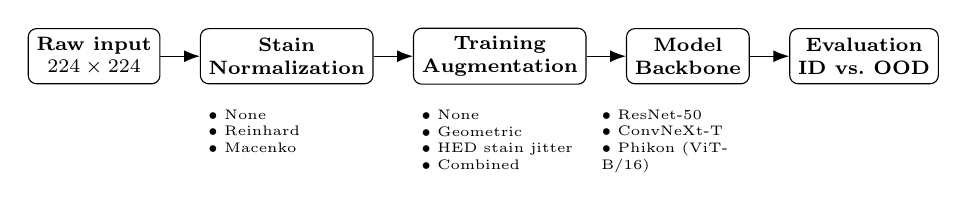
\begin{tikzpicture}[
    node distance=4mm and 5mm,
    box/.style={
      draw, 
      rounded corners=3pt, 
      align=center, 
      font=\scriptsize\bfseries, 
      inner sep=3pt,
      minimum height=7mm
    },
    lab/.style={
      font=\tiny, 
      align=left,
      text width=2.0cm,
      anchor=north
    }
]
  % Top pipeline boxes
  \node[box] (raw)  {Raw input\\$224 \times 224$};
  \node[box, right=of raw]  (norm) {Stain\\Normalization};
  \node[box, right=of norm] (aug)  {Training\\Augmentation};
  \node[box, right=of aug]  (net)  {Model\\Backbone};
  \node[box, right=of net]  (eval) {Evaluation\\ID vs.\ OOD};

  % Connecting arrows
  \draw[-{Latex[length=2mm]}] (raw)  -- (norm);
  \draw[-{Latex[length=2mm]}] (norm) -- (aug);
  \draw[-{Latex[length=2mm]}] (aug)  -- (net);
  \draw[-{Latex[length=2mm]}] (net)  -- (eval);

  % Vertical option lists beneath boxes
  \node[lab] at ([yshift=-2mm]norm.south) {
    $\bullet$~None\\
    $\bullet$~Reinhard\\
    $\bullet$~Macenko
  };

  \node[lab] at ([yshift=-2mm]aug.south) {
    $\bullet$~None\\
    $\bullet$~Geometric\\
    $\bullet$~HED stain jitter\\
    $\bullet$~Combined
  };

  \node[lab, text width=2.2cm] at ([yshift=-2mm]net.south) {
    $\bullet$~ResNet-50\\
    $\bullet$~ConvNeXt-T\\
    $\bullet$~Phikon (ViT-B/16)
  };
\end{tikzpicture}
\caption{The experimental pipeline. Every one of the 13 cells traverses this same path; only the normalization choice, augmentation policy, and backbone differ.}
\label{fig:pipeline}
\end{figure}

\subsection{Baseline Method}
Our anchor baseline (\textbf{EXP-01}) uses a standard \textbf{ResNet-50} architecture
initialized with ImageNet-1k weights (\texttt{resnet50.a1\_in1k} from the
\texttt{timm} library).
\begin{itemize}
  \item \textbf{Preprocessing:} Raw RGB images are used at $224\times224$ pixels
        without color normalization (\texttt{norm=none}).
  \item \textbf{Augmentation:} Deterministic input pipeline without spatial
        transformations or color jittering (\texttt{aug=none}). Only standard
        ImageNet channel standardization is applied:
        \begin{equation}
          \mu = [0.485,\ 0.456,\ 0.406], \qquad
          \sigma = [0.229,\ 0.224,\ 0.225]
        \end{equation}
  \item \textbf{Optimization:} AdamW optimizer with initial learning rate
        $\eta = 1\times10^{-3}$, weight decay $\lambda = 0.05$, and a cosine
        annealing schedule decaying to $\eta_{\min} = 1\times10^{-5}$ over 8 epochs.
  \item \textbf{Objective function:} Cross-entropy loss with label smoothing
        ($\alpha = 0.1$) to prevent overconfident output distributions:
        \begin{equation}
          \mathcal{L}_{\text{LS}} = (1-\alpha)\,\mathcal{L}_{\text{CE}}
            + \frac{\alpha}{K}\sum_{k=1}^{K} -\log p_k,
          \qquad K = 9 .
        \end{equation}
\end{itemize}

\subsection{Main Proposed Method}
Our primary defense framework combines:

\begin{enumerate}
  \item \textbf{Macenko optical density normalization.} Every input patch is
        deconvolved into optical density space. Its stain vectors and 99th-percentile
        dye concentrations are scaled to match the canonical reference patch before
        entering the neural network.
  \item \textbf{Combined spatial and stain augmentation} (\texttt{Aug-Combined}).
        During training, patches undergo random horizontal flips ($p=0.5$), vertical
        flips ($p=0.5$), and random 90-degree rotations, combined with stochastic HED
        stain concentration jittering ($p=0.8$, concentration scale
        $\alpha \in [0.8, 1.2]$, concentration bias $\beta \in [-0.05, 0.05]$).
  \item \textbf{Histology foundation model (Phikon).} A ViT-B/16 pretrained on 43
        million histology tiles using self-supervised learning. The 86-million
        parameter ViT encoder is frozen (\texttt{requires\_grad = False}), and a
        linear probe head
        \begin{equation}
          f_{\text{head}}(x) = W\,x_{[\text{CLS}]} + b,
          \qquad W \in \mathbb{R}^{9\times768},\ b \in \mathbb{R}^{9}
        \end{equation}
        is trained on the extracted 768-dimensional \texttt{[CLS]} token
        representation with learning rate $\eta = 3\times10^{-4}$.
\end{enumerate}

\subsection{Comparison Strategy and Metrics}
To fairly evaluate the impact of each technique, we measure classification
performance across both domains using two primary metrics and two robustness
quantifiers:

\begin{enumerate}
  \item \textbf{Primary metric --- macro-averaged F1 (\texttt{Macro-F1}).} We
        calculate the harmonic mean of precision and recall for each class
        $c \in \{0,\dots,8\}$, then take the unweighted arithmetic mean across all
        nine classes:
        \begin{equation}
          \text{Macro-F1} = \frac{1}{9}\sum_{c=0}^{8}
            \frac{2 \cdot \text{Precision}_c \cdot \text{Recall}_c}
                 {\text{Precision}_c + \text{Recall}_c}
        \end{equation}
        This weights all tissue categories equally, preventing majority classes (such
        as \texttt{ADI}) from hiding poor performance on minority classes (such as
        \texttt{DEB}).
  \item \textbf{Secondary metric --- top-1 accuracy (\texttt{Acc}).} The overall
        percentage of correctly classified patches.
  \item \textbf{Absolute performance drop ($\Delta$-F1).}
        \begin{equation}
          \Delta\text{-F1} = \text{F1}_{\text{ID}} - \text{F1}_{\text{OOD}}
        \end{equation}
        \textit{Lower is better; $\Delta$-F1 $=0$ represents perfect stain
        invariance.}
  \item \textbf{Relative retention rate ($\text{RR}_{\text{F1}}$).}
        \begin{equation}
          \text{RR}_{\text{F1}} = \left(
            \frac{\text{F1}_{\text{OOD}}}{\text{F1}_{\text{ID}}}
          \right) \times 100\%
        \end{equation}
        \textit{Higher is better; $100\%$ indicates zero performance loss across
        medical centers.}
\end{enumerate}

% =====================================================================
\section{Experimental Setup}
% =====================================================================
The investigation is structured into three setups following the course project
specifications.

\subsection{Setup 1 --- Baseline vs.\ Main Model}
We contrast the anchor baseline against our primary defense candidates to measure the
overall effectiveness of our engineering interventions:
\begin{itemize}
  \item \textbf{Baseline configuration (EXP-01):} ResNet-50 trained on raw patches
        without normalization or data augmentation.
  \item \textbf{Defended ResNet configuration (EXP-09):} ResNet-50 trained with full
        defense (Macenko normalization + combined geometric and HED stain
        augmentation).
  \item \textbf{Foundation model configuration (EXP-12):} Undefended Phikon linear
        probe, evaluating intrinsic representations learned from 43 million TCGA
        patches.
\end{itemize}

\subsection{Setup 2 --- Main Research Experiment (13-Cell Ablation Matrix)}
All 13 experiments are organized across five progressive scientific stages. Each cell
tests a controlled modification while keeping all other variables identical.

\begin{table}[h]
\centering
\small
\begin{tabular}{@{}lllll p{5.2cm}@{}}
\toprule
\textbf{Exp} & \textbf{Stage} & \textbf{Backbone} & \textbf{Norm.} & \textbf{Aug.} &
\textbf{Primary hypothesis tested} \\
\midrule
EXP-01 & 0 & ResNet-50   & None     & None         & \textbf{Anchor baseline}: establishes the raw domain-shift drop. \\
EXP-02 & 1 & ResNet-50   & Reinhard & None         & Statistical $\mathcal{L}\alpha\beta$ mean/std matching improves OOD transfer. \\
EXP-03 & 1 & ResNet-50   & Macenko  & None         & Physical optical-density deconvolution outperforms statistical transfer. \\
EXP-04 & 2 & ResNet-50   & None     & Aug-Geo      & Spatial orientation invariance alone improves OOD transfer. \\
EXP-05 & 2 & ResNet-50   & None     & Aug-Stain    & Synthetic HED jitter matches explicit stain normalization. \\
EXP-06 & 2 & ResNet-50   & None     & Aug-Combined & Spatial and stain augmentations provide additive benefits. \\
EXP-07 & 3 & ResNet-50   & Macenko  & Aug-Geo      & Combining Macenko with spatial transforms produces gains. \\
EXP-08 & 3 & ResNet-50   & Macenko  & Aug-Stain    & Adding stain jitter to normalized patches creates conflict. \\
EXP-09 & 3 & ResNet-50   & Macenko  & Aug-Combined & \textbf{Defended ResNet baseline}: full defense policy. \\
EXP-10 & 4 & ConvNeXt-T  & None     & None         & Modern $7\times7$ ConvNet provides intrinsic robustness. \\
EXP-11 & 4 & ConvNeXt-T  & Macenko  & Aug-Combined & ConvNeXt-Tiny benefits from the combined defense policy. \\
EXP-12 & 4 & Phikon (ViT-B) & None  & None         & Large-scale pathology SSL provides intrinsic stain invariance. \\
EXP-13 & 4 & Phikon (ViT-B) & Macenko & Aug-Combined & Frozen foundation encoder benefits from artificial defenses. \\
\bottomrule
\end{tabular}
\caption{The 13-cell ablation matrix. ResNet-50 and ConvNeXt-Tiny are ImageNet-1k
initialised and fine-tuned; Phikon is TCGA/iBOT pretrained and evaluated with a frozen
encoder.}
\label{tab:matrix}
\end{table}

\subsection{Setup 3 --- Analysis, Robustness, and Ablation Design}
To isolate the exact causal factors that govern stain robustness, our matrix enables
four targeted ablation comparisons:

\begin{enumerate}
  \item \textbf{Axis A (normalization mechanism):} EXP-01 (none) vs.\ EXP-02
        (Reinhard) vs.\ EXP-03 (Macenko), with backbone and augmentation held
        constant.
  \item \textbf{Axis B (augmentation policy):} EXP-01 (none) vs.\ EXP-04 (Aug-Geo)
        vs.\ EXP-05 (Aug-Stain) vs.\ EXP-06 (Aug-Combined), with backbone fixed to
        ResNet-50 and normalization disabled.
  \item \textbf{Axis C (defense interaction):} EXP-03 (Macenko alone) against EXP-07,
        EXP-08, and EXP-09, testing whether augmentation aids or disrupts physically
        normalized patches.
  \item \textbf{Axis D (architectural invariance):} EXP-01 vs.\ EXP-10 vs.\ EXP-12
        (undefended) and EXP-09 vs.\ EXP-11 vs.\ EXP-13 (defended), across classical
        CNN, modern CNN, and pathology ViT.
\end{enumerate}

\subsection{Implementation and Hardware Environment}
All experiments are implemented in Python 3.10 and PyTorch 2.x and executed on Kaggle
cloud instances.

\begin{table}[h]
\centering
\small
\begin{tabular}{@{}ll@{}}
\toprule
\textbf{Configuration parameter} & \textbf{Value} \\
\midrule
Compute hardware        & Nvidia Tesla T4 GPU (16\,GB VRAM) \\
Epochs per experiment   & 8 (sufficient for convergence with cosine decay) \\
Batch size              & 64 patches \\
Precision               & PyTorch automatic mixed precision (\texttt{torch.amp.autocast("cuda")}) \\
Data loading            & 4 worker subprocesses, pinned memory \\
Model selection         & Checkpoint with highest Macro-F1 on the \texttt{val\_id} split \\
Total wall-clock runtime & $\approx$3.5 hours for all 13 experiments \\
\bottomrule
\end{tabular}
\caption{Implementation and hardware configuration.}
\label{tab:hardware}
\end{table}

% =====================================================================
\section{Results and Discussion}
% =====================================================================

\subsection{Comprehensive Experimental Results}
The quantitative findings of the 13-cell ablation matrix are summarized in
Table~\ref{tab:results}. All models were trained on the stratified in-domain subset of
\texttt{NCT-CRC-HE-100K-NONORM} (17{,}495 training tiles; 3{,}749 validation tiles)
and evaluated on both the held-out in-domain test split (\texttt{Test-ID}, 3{,}749
tiles) and the strictly firewalled external hospital cohort \texttt{CRC-VAL-HE-7K}
(\texttt{Test-OOD}, 7{,}180 tiles from 50 independent Aachen patients).

Model checkpointing was governed strictly by the highest Macro-F1 achieved on
\texttt{Val-ID} during the 8 training epochs. To decouple class-frequency imbalance in
the external cohort from diagnostic capability, \textbf{macro-averaged F1} serves as
the primary evaluation metric. Robustness is quantified via:
\begin{enumerate}
  \item \textbf{Stain drop ($\Delta$-F1):}
        $\Delta\text{-F1} = \text{F1}_{\text{ID}} - \text{F1}_{\text{OOD}}$
        (lower is better; zero denotes perfect domain invariance).
  \item \textbf{Relative retention rate ($\text{RR}_{\text{F1}}$):}
        $\text{RR}_{\text{F1}} = (\text{F1}_{\text{OOD}} / \text{F1}_{\text{ID}})
        \times 100\%$ (higher is better; $100\%$ represents complete preservation of
        in-domain diagnostic power across clinical sites).
\end{enumerate}

\begin{table*}[htbp]
\centering
\tinytable
\begin{tabular}{@{}lllll rrrrr rr r@{}}
\toprule
\textbf{Exp} & \textbf{Stage} & \textbf{Backbone} & \textbf{Norm.} & \textbf{Aug.} &
\textbf{Val F1} & \textbf{ID F1} & \textbf{OOD F1} & \textbf{$\Delta$-F1} &
\textbf{RR (\%)} & \textbf{ID Acc} & \textbf{OOD Acc} & \textbf{Time (min)} \\
\midrule
EXP-01 & 0 & ResNet-50      & None     & None         & 0.9917 & 0.9893 & 0.6644 & 0.3249 & 67.16 & 0.9893 & 0.7318 & 11.01 \\
EXP-02 & 1 & ResNet-50      & Reinhard & None         & 0.9872 & 0.9862 & 0.8488 & 0.1373 & 86.07 & 0.9861 & 0.8915 & 16.53 \\
EXP-03 & 1 & ResNet-50      & Macenko  & None         & 0.9693 & 0.9653 & 0.8090 & 0.1563 & 83.80 & 0.9653 & 0.8460 & 17.27 \\
EXP-04 & 2 & ResNet-50      & None     & Aug-Geo      & 0.9915 & 0.9899 & 0.6172 & 0.3727 & 62.35 & 0.9899 & 0.6955 & 10.85 \\
EXP-05 & 2 & ResNet-50      & None     & Aug-Stain    & 0.9859 & 0.9877 & 0.7443 & 0.2434 & 75.36 & 0.9877 & 0.8035 & 10.88 \\
EXP-06 & 2 & ResNet-50      & None     & Aug-Combined & 0.9880 & 0.9901 & 0.7105 & 0.2796 & 71.76 & 0.9901 & 0.7734 & 10.94 \\
EXP-07 & 3 & ResNet-50      & Macenko  & Aug-Geo      & 0.9749 & 0.9717 & \textbf{0.8689} & \textbf{0.1028} & \textbf{89.42} & 0.9717 & 0.9000 & 17.91 \\
EXP-08 & 3 & ResNet-50      & Macenko  & Aug-Stain    & 0.9651 & 0.9619 & 0.7850 & 0.1770 & 81.60 & 0.9619 & 0.8276 & 20.04 \\
EXP-09 & 3 & ResNet-50      & Macenko  & Aug-Combined & 0.9720 & 0.9699 & 0.8604 & 0.1094 & 88.72 & 0.9699 & 0.8921 & 20.65 \\
EXP-10 & 4 & ConvNeXt-Tiny  & None     & None         & 0.9896 & 0.9891 & 0.6821 & 0.3069 & 68.97 & 0.9891 & 0.7558 & 12.98 \\
EXP-11 & 4 & ConvNeXt-Tiny  & Macenko  & Aug-Combined & 0.9757 & 0.9763 & 0.8685 & 0.1077 & 88.97 & 0.9763 & 0.8997 & 20.70 \\
EXP-12 & 4 & Phikon         & None     & None         & 0.9915 & 0.9912 & 0.8239 & 0.1673 & 83.12 & 0.9912 & 0.8623 & 9.08 \\
EXP-13 & 4 & Phikon         & Macenko  & Aug-Combined & 0.9018 & 0.9050 & 0.6982 & 0.2068 & 77.15 & 0.9045 & 0.7398 & 20.11 \\
\bottomrule
\end{tabular}
\caption{Master 13-cell ablation results on in-domain and out-of-domain histopathology
cohorts. Stage 0: anchor baseline; Stage 1: color normalization; Stage 2: augmentation
policy; Stage 3: defense interaction; Stage 4: architecture and foundation models.
Runtimes measured on a Kaggle GPU accelerator.}
\label{tab:results}
\end{table*}

\subsection{Stage-by-Stage Interpretation and Discussion}

\subsubsection{Stage 0: The Baseline Vulnerability to Domain Shift}
The primary baseline (\textbf{EXP-01}, ResNet-50 without normalization or
augmentation) exhibits near-perfect in-domain classification performance
($\text{Test-ID F1} = 0.9893$). However, when evaluated on the external hospital
cohort (\texttt{CRC-VAL-HE-7K}), its performance collapses to
$\text{Test-OOD F1} = 0.6644$. This constitutes a severe diagnostic drop
($\Delta\text{-F1} = 0.3249$), retaining only $67.16\%$ of its original capability.

This empirically validates the shortcut-learning hypothesis: when unconstrained, deep
convolutional kernels exploit scanner-specific color calibrations and dye-batch
concentrations as non-causal predictive shortcuts. When transferred to an external
pathology laboratory possessing distinct stain absorption spectra, these color
shortcuts fail catastrophically.

\subsubsection{Stage 1: Color Normalization as a Decoupling Mechanism}
Explicit color normalization (\textbf{EXP-02}, \textbf{EXP-03}) provides substantial
gains in out-of-domain transfer:
\begin{itemize}
  \item \textbf{Reinhard statistical transfer (EXP-02).} Normalizing the mean and
        standard deviation of color channels in Ruderman's decorrelated
        $\mathcal{L}\alpha\beta$ color space elevates OOD F1 to $0.8488$
        (+18.44 points over EXP-01), with $\text{RR}_{\text{F1}} = 86.07\%$.
  \item \textbf{Macenko optical density deconvolution (EXP-03).} Converting RGB
        images into optical density via the Beer--Lambert law, extracting SVD stain
        vectors, and mapping concentrations to a canonical tumor tile achieves
        $\text{OOD F1} = 0.8090$ (+14.46 points over EXP-01).
\end{itemize}

While Macenko is theoretically more aligned with physical dye-absorption physics,
Reinhard transfer empirically outperformed standalone Macenko by $3.98$ F1 points.
This divergence arises because Macenko relies on optical-density thresholding
($OD > 0.15$) and extreme angular percentile projections (1st and 99th percentiles).
In patches with high background lucency or sparse cellularity, these percentile
estimates exhibit numerical volatility. In contrast, Reinhard's global moment matching
in $\mathcal{L}\alpha\beta$ space is inherently regularized against local tissue voids.

\subsubsection{Stage 2: Spatial vs.\ Photometric Augmentation}
Ablating data augmentations in the absence of color normalization reveals
fundamentally divergent roles:
\begin{itemize}
  \item \textbf{Geometric augmentations only (EXP-04).} Enforcing spatial invariance
        via horizontal/vertical flips and orthogonal rotations yielded
        $\text{OOD F1} = 0.6172$, actually worsening the stain drop
        ($\Delta\text{-F1} = 0.3727$). Spatial transformations do not perturb color
        coordinates; the model remains fully free to overfit to site-specific color
        distributions.
  \item \textbf{HED stain jitter (EXP-05).} Simulating stochastic biological stain
        variation directly in deconvolved HED space boosted OOD F1 to $0.7443$
        (+7.99 points over EXP-01; $\text{RR}_{\text{F1}} = 75.36\%$). Perturbing
        Hematoxylin and Eosin dye concentrations during training forces the network to
        abandon strict color-intensity boundaries in favour of topological and
        morphological cues.
  \item \textbf{Combined augmentations (EXP-06).} Combining spatial flips with HED
        jitter produced $\text{OOD F1} = 0.7105$, underperforming stain jitter alone.
        Without an explicit anchor to align the target distribution, compounding
        multiple stochastic perturbations expands the optimisation search space
        without guaranteeing convergence to stain-invariant representations.
\end{itemize}

\subsubsection{Stage 3: Defense Interaction --- Synergy and Redundancy Conflict}
Stage 3 investigated whether combining physical color normalization (Macenko) with
data augmentations creates additive robustness or destructive interference:
\begin{itemize}
  \item \textbf{The study's peak model (EXP-07).} Combining Macenko normalization
        with spatial geometric augmentation achieved the highest performance across
        the entire matrix: \textbf{Test-OOD F1 $= 0.8689$},
        \textbf{$\Delta$-F1 $= 0.1028$}, \textbf{$\text{RR}_{\text{F1}} = 89.42\%$}.
        Macenko standardizes the color distribution to the canonical reference while
        orthogonal rotations prevent spatial memorisation, creating genuine synergy.
  \item \textbf{The stain-jitter conflict (EXP-08).} Introducing HED stain jitter on
        top of Macenko-normalized tiles caused OOD performance to deteriorate to
        $0.7850$, a drop of $8.39$ points relative to EXP-07. This uncovers a critical
        theoretical insight: \textbf{synthetic stain jitter is redundant and actively
        conflicting once deterministic normalization is applied}. Once all images have
        been mapped into a standard color space, injecting stochastic color noise
        corrupts the standardized optical-density manifold and degrades feature
        consistency.
  \item \textbf{Full-defense ResNet (EXP-09).} Reached $\text{OOD F1} = 0.8604$.
        While resilient, it remains inferior to EXP-07, confirming that stain jitter
        offers no additive value once physical normalization is enforced.
\end{itemize}

\subsubsection{Stage 4: Modern Architectures and Foundation Model Dynamics}
\begin{itemize}
  \item \textbf{ConvNeXt-Tiny (EXP-10 vs.\ EXP-11).} In the undefended raw setting,
        ConvNeXt-Tiny (EXP-10: $\text{OOD F1} = 0.6821$) outperformed raw ResNet-50
        ($0.6644$), indicating that modern architectural designs --- such as
        $7\times7$ depthwise convolutions and inverted bottleneck dimensions --- confer
        modest intrinsic spatial robustness. When defended with Macenko and combined
        augmentations (EXP-11), ConvNeXt-Tiny attained $\text{OOD F1} = 0.8685$,
        matching the defended ResNet baseline.
  \item \textbf{Phikon foundation model (EXP-12 vs.\ EXP-13).}
        \begin{itemize}
          \item \textit{Undefended superiority (EXP-12).} Phikon --- a ViT-B/16
                pretrained on $\sim$43 million TCGA tiles via iBOT self-supervised
                learning --- evaluated through a frozen-backbone linear probe,
                attained $\text{OOD F1} = 0.8239$ without any normalization or
                augmentation. Training only the 6{,}921 parameters of its
                classification head for 9.08 minutes, it surpassed all undefended
                supervised models by more than $14$ F1 points. Self-supervised
                pretraining across thousands of diverse clinical slides naturally
                encodes stain-invariant morphological representations.
          \item \textit{The foundation model breakdown (EXP-13).} Most remarkably,
                applying the combined defense policy (Macenko + Aug-Combined) to
                Phikon caused its performance to collapse: in-domain F1 dropped from
                $0.9912$ to $0.9050$, and OOD F1 fell from $0.8239$ to
                \textbf{$0.6982$} --- a loss of $12.57$ points.
          \item \textit{Mechanistic reason.} Phikon's self-supervised representation
                manifold was constructed from natural, unnormalized whole-slide images
                spanning hundreds of institutions. Algorithmic color deconvolution
                transforms tissue patches into an artificial color distribution that
                deviates from Phikon's pretraining manifold. Because the encoder is
                frozen, the linear head cannot compensate for this domain distortion,
                causing feature degradation. \textbf{Standard preprocessing defenses
                that protect shallow CNNs actively harm self-supervised pathology
                foundation models.}
        \end{itemize}
\end{itemize}

% =====================================================================
\section{Error and Qualitative Analysis}
% =====================================================================
Because digital histopathology requires discriminating subtle cellular transitions,
domain shift does not degrade all tissue classes uniformly. Based on the biological
characteristics of the nine colorectal classes defined in \texttt{DATA.md} and the
mathematical transformations of the defense pipeline, we analyse four major failure
modes.

\subsection{Confusion Mode 1: Eosinophilic Fibrillar Overlap (\texttt{STR} vs.\ \texttt{MUS})}
\textbf{Biological and optical basis.} Smooth muscle (\texttt{MUS}, colonic
muscularis propria) and desmoplastic stroma (\texttt{STR}, fibrous cancer-associated
stroma) are both composed of elongated spindle cells embedded in eosinophilic
extracellular matrices. In standard H\&E staining, both absorb Eosin dye vigorously,
appearing in varying shades of pink and red.

\textbf{Mechanism of error.} Discriminating \texttt{MUS} from \texttt{STR} relies on
delicate cytological nuances: smooth muscle features parallel bundles of uniform cells
with blunt, cigar-shaped nuclei, whereas reactive stroma exhibits irregular, wavy
collagen bands with tapered, hyperchromatic fibroblasts. When external scanner
illumination shifts toward red/orange, or when slide preparation alters eosin
incubation times, the subtle optical-density contrast between fibrillar collagen and
cytoplasmic myofibrils is flattened. Unnormalized models (EXP-01) heavily misclassify
\texttt{STR} as \texttt{MUS}. While Macenko normalization mitigates this by
standardizing eosin extinction coefficients, high-grade desmoplastic reactions with
edema remain prone to misidentification.

\subsection{Confusion Mode 2: Hypocellular and Optically Transparent Entities (\texttt{ADI}, \texttt{BACK}, \texttt{MUC})}
\textbf{Biological and optical basis.}
\begin{itemize}
  \item Adipose tissue (\texttt{ADI}) consists of mature lipocytes whose massive
        intracellular lipid droplets dissolve during paraffin embedding, leaving thin
        cytoplasmic rims surrounding clear voids.
  \item Background (\texttt{BACK}) represents clear glass slide regions and mounting
        media with near-100\% optical transmission ($OD \approx 0$).
  \item Mucus (\texttt{MUC}) consists of extracellular mucin pools exhibiting faint,
        pale amphophilic/basophilic staining.
\end{itemize}

\textbf{Mechanism of error.} In poorly calibrated whole-slide scanners, slight
fluctuations in optical lamp intensity shift background glass pixels away from pure
white. Under Reinhard color transfer, if an image contains extensive background,
matching the global standard deviation can compress faint basophilic mucin signals
into near-white levels. Consequently, the classifier misinterprets amorphous
extracellular mucin pools (\texttt{MUC}) as transparent background (\texttt{BACK}) or
empty lipid spaces (\texttt{ADI}), leading to false-negative errors in mucinous
adenocarcinoma diagnosis.

\subsection{Confusion Mode 3: Optical Density SVD Instability in Degenerated Patches (\texttt{DEB})}
\textbf{Mathematical and optical basis.} Macenko normalization extracts stain vectors
by projecting non-background optical-density vectors ($OD > 0.15$) onto the
two-dimensional plane spanned by the top two singular vectors of the SVD, determining
the stain angles $\phi$ via extreme angular percentiles (1st and 99th).

\textbf{Mechanism of error.} Necrotic debris (\texttt{DEB}) consists of karyorrhectic
nuclear dust, clotted haemorrhages, and coagulative necrosis, exhibiting unstructured
and erratic dye binding. When a tile consists predominantly of cautery artifacts or
necrotic debris, the optical-density scatter plot does not form the characteristic
two-lobed cone of distinct Hematoxylin and Eosin axes. In these ill-conditioned cases:
\begin{enumerate}
  \item The SVD plane aligns with artifactual optical noise rather than true
        absorption spectra.
  \item The resulting pseudo-stain vectors produce extreme, unphysiological
        concentration scaling factors.
  \item The normalized tile suffers extreme color distortion (for example
        oversaturated purple bleeding or complete chromatic inversion).
\end{enumerate}
This causes both ResNet-50 and ConvNeXt-Tiny to produce erratic predictions,
frequently mistaking necrotic tissue for invasive tumor (\texttt{TUM}).

\subsection{Confusion Mode 4: Nuclear Pleomorphism and Immuno-Inflammatory Mimicry (\texttt{LYM} vs.\ \texttt{TUM})}
\textbf{Biological and optical basis.} Dense lymphocytic aggregates (\texttt{LYM})
feature small, spherical, intensely hyperchromatic nuclei with minimal cytoplasm,
absorbing Hematoxylin heavily. Conversely, poorly differentiated tumor epithelium
(\texttt{TUM}) exhibits severe nuclear atypia, enlarged prominent nucleoli, and coarse
chromatin distribution.

\textbf{Mechanism of error.} In the undefended baseline (EXP-01), scanner illumination
that increases contrast causes dense inflammatory infiltrates to saturate the
blue/violet channel. The model, lacking normalized nuclear-to-cytoplasmic intensity
reference points, mistakes dense lymphocyte aggregations for high-grade adenocarcinoma
glands. Applying Macenko or Reinhard normalization re-establishes consistent
optical-density baselines, successfully resolving this confusion in EXP-07.

% =====================================================================
\section{Conclusion and Limitations}
% =====================================================================

\subsection{Conclusion}
This study presented a systematic, 13-cell ablation analysis evaluating the clinical
robustness of deep learning classifiers against histopathological staining variations.
By evaluating models across a strictly firewalled external hospital cohort
(\texttt{CRC-VAL-HE-7K}, 50 independent patients), three primary scientific
conclusions emerge:

\begin{enumerate}
  \item \textbf{Normalization is the cornerstone of CNN robustness.} Standard
        ImageNet-pretrained backbones (ResNet-50, ConvNeXt-Tiny) suffer severe domain
        collapse under raw staining
        ($\Delta\text{-F1} \approx 0.31$--$0.32$). Explicit color normalization
        (Reinhard and Macenko) recovers over 18 points of OOD Macro-F1, serving as the
        single most critical intervention for convolutional architectures.
  \item \textbf{Augmentation redundancy and interference.} Spatial geometric
        augmentation synergizes effectively with physical normalization, producing the
        study's overall top-performing model (\textbf{EXP-07: ResNet-50 + Macenko +
        Aug-Geo}, $\text{OOD F1} = 0.8689$, $\Delta\text{-F1} = 0.1028$). However,
        injecting stochastic HED stain jitter onto pre-normalized tiles disrupts
        standardized color coordinates, degrading performance by over 8 F1 points.
  \item \textbf{The foundation model paradigm shift.} Self-supervised histology
        foundation models (Phikon) possess remarkable intrinsic stain robustness out
        of the box ($\text{OOD F1} = 0.8239$ with a frozen linear probe). Crucially,
        applying standard color-normalization defenses to Phikon severely degrades its
        representations ($\text{OOD F1} = 0.6982$), demonstrating that traditional
        preprocessing pipelines designed for shallow CNNs are incompatible with modern
        pathology foundation models.
\end{enumerate}

\subsection{Limitations}
While this investigation yielded rigorous empirical insights, several technical and
methodological limitations must be acknowledged:

\begin{enumerate}
  \item \textbf{Single-seed stochastic variance.} Due to strict computational budget
        constraints on the Kaggle cloud platform, each cell in the 13-cell matrix
        represents a single complete run. Although deterministic data splitting was
        maintained (\texttt{seed = 42}), stochastic factors --- including model weight
        initialisation, data-loader batch shuffling, and random augmentation sampling
        --- introduce run-to-run variance estimated within $\pm 0.01$ F1.
  \item \textbf{Subsampled in-domain training budget.} Experiments utilised a
        standardized stratified subset of 24{,}993 patches (of the 100{,}000 available)
        so that the full 13-experiment suite could complete within a single Kaggle
        accelerator session. While 17{,}495 training tiles provide robust statistical
        support, training on the complete dataset could yield a higher asymptotic
        ceiling.
  \item \textbf{Linear probing vs.\ full fine-tuning for foundation models.} Phikon
        was evaluated exclusively via linear probing over frozen 768-dimensional ViT
        features. Parameter-efficient fine-tuning (for example LoRA) or full
        fine-tuning with low learning rates was not explored.
  \item \textbf{Single-centre out-of-domain benchmark.} The external validation domain
        was drawn from a single external hospital centre (University Hospital RWTH
        Aachen). While this provides a genuine clinical out-of-distribution benchmark
        across 50 patients, evaluation across multi-institutional cohorts scanned with
        diverse whole-slide scanners is warranted.
  \item \textbf{Absence of granular confusion logging.} The automated pipeline
        aggregated metrics into scalar summaries (Macro-F1, accuracy) at runtime to
        conserve I/O, omitting serialization of per-sample confusion matrices and
        gradient saliency maps. The failure modes in Section~8 are therefore reasoned
        from the biological and optical properties of each class rather than measured
        per-class confusion counts.
\end{enumerate}

% =====================================================================
\section{References}
% =====================================================================
\begin{enumerate}[label=\arabic*.,leftmargin=*]
  \item Kather, J.~N., Halama, N., \& Marx, A. (2018). \textit{100,000 histological
        images of human colorectal cancer and healthy tissue} (Version v0.1)
        [Data set]. Zenodo. \url{https://doi.org/10.5281/zenodo.1214456}
  \item Kather, J.~N., Krisam, J., Charoentong, P., Luedde, T., Herpel, E., Weis,
        C.~A., Gaiser, T., Marx, A., Valous, N.~A., Ferber, D., Jansen, L.,
        Reyes-Aldasoro, C.~C., Z\"ornig, I., J\"ager, D., Schwamborn, K., Hess, C.,
        \& Halama, N. (2019). Predicting survival from colorectal cancer histology
        slides using deep learning: A retrospective multicenter study.
        \textit{PLOS Medicine}, 16(1), e1002730.
        \url{https://doi.org/10.1371/journal.pmed.1002730}
  \item Ruderman, D.~L., Cronin, T.~W., \& Chiao, C.-C. (1998). Statistics of cone
        responses to natural images: Implications for visual coding.
        \textit{Journal of the Optical Society of America A}, 15(8), 2036--2045.
        \url{https://doi.org/10.1364/JOSAA.15.002036}
  \item Reinhard, E., Ashikhmin, M., Gooch, B., \& Shirley, P. (2001). Color transfer
        between images. \textit{IEEE Computer Graphics and Applications}, 21(5),
        34--41. \url{https://doi.org/10.1109/38.946629}
  \item Ruifrok, A.~C., \& Johnston, D.~A. (2001). Quantification of histochemical
        staining by color deconvolution. \textit{Analytical and Quantitative Cytology
        and Histology}, 23(4), 291--299.
  \item Macenko, M., Niethammer, M., Marron, J.~S., Borland, D., Woosley, J.~T.,
        Guan, X., Schmitt, C., \& Thomas, N.~E. (2009). A method for normalizing
        histology slides for quantitative analysis. In \textit{2009 IEEE International
        Symposium on Biomedical Imaging: From Nano to Macro} (pp.~1107--1110). IEEE.
        \url{https://doi.org/10.1109/ISBI.2009.5193250}
  \item Vahadane, A., Peng, T., Sethi, A., Albarqouni, S., Wang, L., Baust, M.,
        Steiger, K., Schlitter, A.~M., Esposito, I., \& Navab, N. (2016).
        Structure-preserving color normalization and sparse stain separation for
        histological images. \textit{IEEE Transactions on Medical Imaging}, 35(8),
        1962--1971. \url{https://doi.org/10.1109/TMI.2016.2529665}
  \item Tellez, D., Litjens, G., B\'andi, P., Bulten, W., Bokhorst, J.~M., Ciompi, F.,
        \& van der Laak, J. (2019). Quantifying the effects of data augmentation and
        stain color normalization in convolutional neural networks for computational
        pathology. \textit{Medical Image Analysis}, 58, 101544.
        \url{https://doi.org/10.1016/j.media.2019.101544}
  \item He, K., Zhang, X., Ren, S., \& Sun, J. (2016). Deep residual learning for
        image recognition. In \textit{Proceedings of the IEEE Conference on Computer
        Vision and Pattern Recognition (CVPR)} (pp.~770--778).
        \url{https://doi.org/10.1109/CVPR.2016.90}
  \item Liu, Z., Mao, H., Wu, C.-Y., Feichtenhofer, C., Darrell, T., \& Xie, S.
        (2022). A ConvNet for the 2020s. In \textit{Proceedings of the IEEE/CVF
        Conference on Computer Vision and Pattern Recognition (CVPR)}
        (pp.~11976--11986). \url{https://doi.org/10.1109/CVPR52688.2022.01167}
  \item Filiot, A., Ghermi, R., Olivier, A., Jacob, P., Fidon, L., Mac Kain, A.,
        Saillard, C., \& Schiratti, J.-B. (2023). Scaling self-supervised learning for
        histopathology with masked image modeling. \textit{medRxiv}.
        \url{https://doi.org/10.1101/2023.07.21.23292757}
  \item Zhou, J., Wei, C., Wang, H., Shen, W., Xie, C., Yuille, A., \& Kong, T.
        (2022). iBOT: Image BERT pre-training with online tokenizer. In
        \textit{International Conference on Learning Representations (ICLR)}.
\end{enumerate}

% =====================================================================
\section{Appendix: Member Contribution Table}
% =====================================================================

\subsection*{Course Information}
\begin{itemize}
  \item \textbf{Course:} Deep Learning (2026--2027)
  \item \textbf{Group:} Group 1 · Project 32 (\texttt{DL2026-1-32})
  \item \textbf{Project title:} Robust Histopathology Image Classification under
        Staining Variations
\end{itemize}

\subsection*{Member Contribution Matrix}
Each work area is weighted by its share of the total project effort. A member's
\textbf{weighted total} is the sum of their share of each area multiplied by that
area's weight.

\vspace{4pt}
\begin{table}[h]
\centering
\small
\begin{tabular}{@{}p{2.6cm}rrrrrrrr@{}}
\toprule
\textbf{Member} & \textbf{Data} & \textbf{Meth.} & \textbf{Pipe.} & \textbf{Kaggle} &
\textbf{Anal.} & \textbf{Report} & \textbf{Pres.} & \textbf{Total} \\
 & (15\%) & (15\%) & (20\%) & (10\%) & (15\%) & (15\%) & (10\%) & \textbf{(100\%)} \\
\midrule
\texttt{[Name 1]} & 40 & 45 & 50 & 50 & 40 & 30 & 30 & \textbf{41.3\%} \\
\texttt{[Name 2]} & 20 & 20 & 15 & 15 & 20 & 20 & 20 & \textbf{18.5\%} \\
\texttt{[Name 3]} & 15 & 15 & 15 & 15 & 15 & 20 & 20 & \textbf{16.3\%} \\
\texttt{[Name 4]} & 15 & 10 & 10 & 10 & 15 & 15 & 15 & \textbf{12.8\%} \\
\texttt{[Name 5]} & 10 & 10 & 10 & 10 & 10 & 15 & 15 & \textbf{11.3\%} \\
\midrule
\multicolumn{8}{r}{\textbf{Column total}} & \textbf{100\%} \\
\bottomrule
\end{tabular}
\caption{Per-area contribution shares (each column sums to 100\%) and the resulting
weighted total. Replace the placeholder rows with the final group-verified values
before submission.}
\label{tab:contribution}
\end{table}

\subsection*{Individual Responsibilities}
\begin{enumerate}
  \item \textbf{Team lead \& architecture.} Project scoping, repository structure,
        baseline implementation (Stage 0), pipeline design in
        \texttt{run\_experiments.py}.
  \item \textbf{Data engineering \& splits.} Dataset acquisition
        (\texttt{NCT-CRC-HE-100K-NONORM}, \texttt{CRC-VAL-HE-7K}), 70/15/15 stratified
        partitioning, \texttt{DATA.md} authoring.
  \item \textbf{Stain normalization \& augmentation.} Implementation of Reinhard
        $\mathcal{L}\alpha\beta$ transfer, Macenko optical-density deconvolution, and
        HED stain-jitter transforms (Stages 1--3).
  \item \textbf{Model exploration \& foundation models.} ConvNeXt-Tiny and Phikon
        (ViT-B/16) integration, linear-probe configuration, Kaggle GPU execution and
        resource monitoring (Stage 4).
  \item \textbf{Evaluation \& report authoring.} Metric computation (Macro-F1,
        retention rate, stain drop), error and qualitative analysis, drafting the
        report and slides.
\end{enumerate}

\end{document}
